


\begin{frame}[fragile]
\frametitle{Internals}

 \begin{block}{Vector Addition}
  \begin{lstlisting}
 x = y + z;
  \end{lstlisting}
 \end{block}

  %\pause

 \begin{block}{Naive Operator Overloading}
  \begin{lstlisting}
 vector<T> operator+(vector<T> & v, vector<T> & w);
  \end{lstlisting}

  %\pause

  \begin{itemize}
   \item t $\leftarrow$ y + z, x $\leftarrow$ t
   %\pause
   \item Temporaries are extremely expensive! 
  \end{itemize}
 \end{block}

   %\pause

 \begin{block}{Expression Templates}
  \begin{lstlisting}
 vector_expr<vector<T>, op_plus, vector<T> >
 operator+(vector<T> & v, vector<T> & w) { ... }

 vector::operator=(vector_expr<...> const & e) {
   viennacl::linalg::avbv(*this, 1,e.lhs(), 1,e.rhs());
 }
  \end{lstlisting}
  \vspace*{0.5cm}

 \end{block}

\end{frame}



\begin{frame}[fragile]
\frametitle{Internals}

 \begin{block}{Vector Addition}
  \begin{lstlisting}
// x = y + z
void avbv(...) {
  switch (active_handle_id(x))
  {
    case MAIN_MEMORY:
      host_based::avbv(...);
      break;
    case OPENCL_MEMORY:
      opencl::avbv(...);
      break;
    case CUDA_MEMORY:
      cuda::avbv(...);
      break;
    default: 
      raise_error();
  }
}
\end{lstlisting}
  \begin{itemize}
   \item Memory buffers can switch memory domain at runtime
  \end{itemize}

 \end{block}

\end{frame}

\begin{frame}[fragile]
\frametitle{Internals}

 \begin{block}{Memory Buffer Migration}
  \begin{lstlisting}
  vector<double> x = zero_vector<double>(42);

  memory_types src_memory_loc = memory_domain(x);
  switch_memory_domain(x, MAIN_MEMORY);

  /* do work on x in main memory here */

  switch_memory_domain(x, src_memory_loc);
\end{lstlisting}

  \begin{center}
    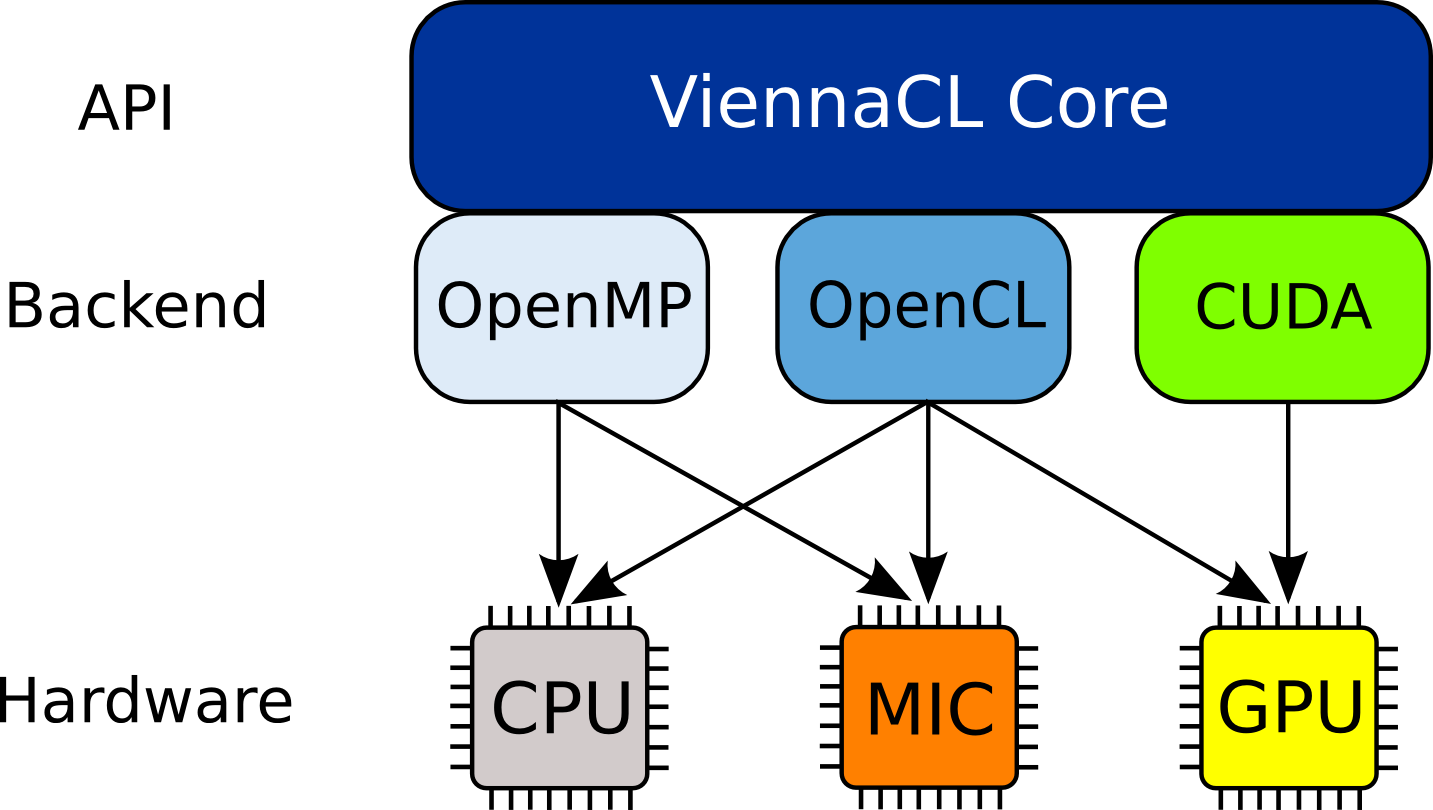
\includegraphics[width=0.6\textwidth]{figures/ViennaCL-arch.png}
  \end{center}
 \end{block}

\end{frame}




\begin{frame}[fragile]
\frametitle{Internals}

 \begin{block}{Generalizing compute kernels}
  \begin{lstlisting}
  // x = y + z
  __kernel void avbv(
    double * x,

    double * y,

    double * z, uint size)
{
  for (size_t i  = get_global_id(0);
              i  < size;
              i += get_global_size())
    x[i] = y[i] + z[i]; 

}
  \end{lstlisting}
 \end{block}

 \vspace*{1.5cm}
\end{frame}



\begin{frame}[fragile]
\frametitle{Internals}

 \begin{block}{Generalizing compute kernels}
  \begin{lstlisting}
  // x = a * y + b * z
  __kernel void avbv(
    double * x,
    double a,
    double * y,
    double b,
    double * z, uint size)
{
  for (size_t i  = get_global_id(0);
              i  < size;
              i += get_global_size())
    x[i] = a * y[i] + b * z[i]; 

}
  \end{lstlisting}
 \end{block}

 \vspace*{1.5cm}
\end{frame}


\begin{frame}[fragile]
\frametitle{Internals}

 \begin{block}{Generalizing compute kernels}
  \begin{lstlisting}
  // x[4:8] = a * y[2:6] + b * z[3:7]
  __kernel void avbv(
    double * x, uint off_x,
    double a,
    double * y, uint off_y,
    double b,
    double * z, uint off_z, uint size)
{
  for (size_t i  = get_global_id(0);
              i  < size;
              i += get_global_size())
    x[off_x + i] = a * y[off_y + i] + b * z[off_z + i]; 

}
  \end{lstlisting}
 \end{block}

 \vspace*{1.5cm}
\end{frame}



\begin{frame}[fragile]
\frametitle{Internals}

 \begin{block}{Generalizing compute kernels}
  \begin{lstlisting}
  // x[4:2:8] = a * y[2:2:6] + b * z[3:2:7]
  __kernel void avbv(
    double * x, uint off_x, uint inc_x,
    double a,
    double * y, uint off_y, uint inc_y,
    double b,
    double * z, uint off_z, uint inc_z, uint size)
{
  for (size_t i  = get_global_id(0);
              i  < size;
              i += get_global_size())
    x[off_x + i * inc_x] =  a * y[off_y + i * inc_y]
                          + b * z[off_z + i * inc_z]; 
}
  \end{lstlisting}
 \end{block}

  \begin{block}{}
   \begin{itemize}
    \item No penalty on GPUs because FLOPs are for free
   \end{itemize}
  \end{block}

\end{frame}


